% CTU-Chat: Asymmetric Multi-Agent Agentic RAG with Knowledge Graph
% for Vietnamese University Counseling
% Springer LNCS format — Paper v2 (revised per advisor feedback)

\documentclass[runningheads]{llncs}

\usepackage[T1]{fontenc}
\usepackage[utf8]{inputenc}
\usepackage{graphicx}
\usepackage{amsmath,amssymb}
\usepackage{algorithm}
\usepackage[noend]{algpseudocode}
\usepackage{booktabs}
\usepackage{multirow}
\usepackage{hyperref}
\usepackage{tikz}
\usetikzlibrary{shapes.geometric, arrows.meta, positioning, fit, calc}
\usepackage{subcaption}
\usepackage{xcolor}

% Custom colors for diagrams
\definecolor{supervisorblue}{HTML}{2563EB}
\definecolor{academicblue}{HTML}{3B82F6}
\definecolor{financialyellow}{HTML}{EAB308}
\definecolor{scholarshippurple}{HTML}{8B5CF6}
\definecolor{generalorange}{HTML}{F97316}
\definecolor{retrievalgreen}{HTML}{22C55E}

\begin{document}

\title{CTU-Chat: Asymmetric Multi-Agent Agentic RAG\\with Knowledge Graph for Vietnamese\\University Counseling}

\author{Cao Tuong Hung\inst{1}}

\authorrunning{C.T.~Hung}

\institute{Can Tho University, Can Tho, Vietnam\\
\email{hungb2303873@student.ctu.edu.vn}}

\maketitle

% ============================================================
% ABSTRACT
% ============================================================
\begin{abstract}
University student-service chatbots must accurately handle diverse query types---from relational academic-program lookups to exact tuition calculations and open-ended policy questions---yet existing Retrieval-Augmented Generation (RAG) systems treat all queries uniformly, wasting computation on simple questions and lacking precision on complex ones.
This paper presents \textbf{CTU-Chat}, a Vietnamese university counseling system built on three novel contributions:
(i)~an \emph{Asymmetric Multi-Agent} architecture that assigns differentiated autonomy levels---full ReAct reasoning, context-bounded ReAct, or zero-shot chain---to specialist agents based on query complexity;
(ii)~\emph{Intent-Guided Subspace Retrieval Routing} (IG-SRR), which couples LLM intent classification with deterministic metadata lane filters to confine hybrid retrieval (BM25~+~dense vector~+~RRF~+~cross-encoder reranking) to ontologically correct document subspaces; and
(iii)~a \emph{Neo4j Knowledge Graph} with typed Python tools that eliminates schema hallucination by replacing raw Cypher generation with safe, parameterized graph queries.
The system is implemented with LangGraph, Qdrant, Neo4j, and Gemini, and evaluated on a 100-question Vietnamese benchmark spanning four domains.
Preliminary results show 91\% LLM-judge pass rate, 96.67\% tool-calling accuracy, and 100\% expected-source coverage across reranker variants.
Controlled retrieval ablations and RAGAS-based answer-quality evaluations are in progress.

\keywords{Retrieval-Augmented Generation \and Multi-Agent Systems \and Knowledge Graph \and Vietnamese NLP \and University Chatbot \and LangGraph}
\end{abstract}

% ============================================================
% 1. INTRODUCTION
% ============================================================
\section{Introduction}
\label{sec:introduction}

% --- Topic Introduction ---
The rapid expansion of higher education enrollment in Vietnam has placed unprecedented pressure on university administrative offices to respond to student inquiries regarding academic programs, tuition fees, scholarships, and institutional policies~\cite{lewis2020rag}. Can Tho University (CTU), the largest institution in the Mekong Delta region, serves tens of thousands of students across more than 100 academic programs, generating a constant stream of diverse counseling requests. Traditional FAQ-based or rule-based chatbots have proven inadequate: they cannot reason over relational academic structures, perform precise financial calculations, or adapt to annually changing regulations.

% --- Topic Background ---
Retrieval-Augmented Generation (RAG)~\cite{lewis2020rag} has emerged as the dominant paradigm for grounding large language models (LLMs) in external knowledge. Recent advances have extended basic RAG along two axes. First, \emph{hybrid retrieval} pipelines combine sparse lexical search (BM25~\cite{robertson2009bm25}) with dense vector embeddings and reciprocal-rank fusion (RRF~\cite{cormack2009rrf}) to capture both keyword precision and semantic similarity. Second, \emph{Agentic RAG} integrates autonomous agents capable of tool use, multi-step reasoning, and dynamic planning into the retrieval--generation loop. Knowledge Graph RAG (GraphRAG)~\cite{edge2024graphrag} further augments this paradigm by leveraging graph-structured knowledge for relational queries that flat document retrieval cannot answer.

% --- Research Problem (Research Gaps) ---
Despite these advances, deploying Agentic GraphRAG systems in domain-specific educational settings reveals five critical research gaps identified in recent literature:

\begin{enumerate}
    \item \textbf{Schema hallucination and tool overload}: When LLM agents generate raw Cypher queries against knowledge graphs, they frequently produce syntactically valid but semantically incorrect queries, especially on complex schemas with many relationship types~\cite{edge2024graphrag}.
    \item \textbf{Latency and computational overhead}: Homogeneous multi-agent architectures that assign full ReAct reasoning loops to every query---including trivial ones---consume excessive LLM tokens and introduce unacceptable latency for real-time counseling~\cite{yao2023react}.
    \item \textbf{Score-space incompatibility in hybrid fusion}: BM25 scores, dense cosine similarities, and graph topology signals occupy fundamentally different mathematical spaces, making na\"ive fusion via static RRF suboptimal.
    \item \textbf{Temporal knowledge degradation}: Static knowledge graphs cannot track annually changing tuition rates, admission criteria, or scholarship policies without costly full recomputation.
    \item \textbf{Lack of multi-agent evaluation frameworks}: Standard end-result metrics (BLEU, ROUGE, or single-turn RAGAS) are blind to agent coordination quality, tool-call validity, and routing accuracy.
\end{enumerate}

% --- Research Objective ---
This paper addresses Gaps~1--3 directly and proposes partial solutions for Gap~5. Specifically, we present \textbf{CTU-Chat}, a Vietnamese university counseling system with three core contributions:

\begin{itemize}
    \item An \textbf{Asymmetric Multi-Agent} architecture implemented via LangGraph's Supervisor Pattern, where each specialist agent receives a differentiated autonomy level matched to the inherent complexity of its domain (Section~\ref{sec:asymmetric}).
    \item \textbf{Intent-Guided Subspace Retrieval Routing (IG-SRR)}, a mechanism that couples LLM-based intent classification with deterministic metadata lane filters, confining hybrid BM25\,+\,dense retrieval to ontologically correct document subspaces before RRF fusion (Section~\ref{sec:igssr}).
    \item \textbf{Typed Knowledge Graph tools} for Neo4j that replace unconstrained Cypher generation with safe, parameterized Python functions, eliminating schema hallucination at the architectural level (Section~\ref{sec:kg}).
\end{itemize}

% --- Research Methodology ---
The system is built with FastAPI, LangGraph, Qdrant vector database, Neo4j graph database, Redis session memory, PostgreSQL persistent storage, and Google Gemini LLMs. We evaluate on a curated 100-question Vietnamese benchmark balanced across four domains: tuition, exemption/social-support, scholarships, and student loans.

% --- Paper Outline ---
The remainder of this paper is organized as follows. Section~\ref{sec:related} reviews related work on RAG, knowledge graphs, and multi-agent systems, identifying the research gaps that motivate our design. Section~\ref{sec:proposed} presents the proposed model in detail, including system architecture, agent design, retrieval pipeline, and routing algorithms. Section~\ref{sec:experiments} describes the experimental setup, evaluation metrics, and results. Section~\ref{sec:conclusion} concludes the paper and outlines future directions.


% ============================================================
% 2. RELATED WORK
% ============================================================
\section{Related Work}
\label{sec:related}

\subsection{Retrieval-Augmented Generation and Hybrid Search}
\label{sec:rag_hybrid}

Lewis et al.~\cite{lewis2020rag} introduced RAG as a method to ground LLM outputs in retrieved documents, significantly reducing hallucination. The standard dense retrieval pipeline encodes queries and documents into a shared vector space and retrieves by cosine similarity. However, dense retrieval alone struggles with exact keyword matches, abbreviations, and Vietnamese compound nouns.

BM25~\cite{robertson2009bm25} addresses these shortcomings through sparse lexical matching with term-frequency saturation and document-length normalization. Hybrid retrieval systems combine both approaches. Reciprocal Rank Fusion (RRF)~\cite{cormack2009rrf} merges ranked lists without requiring score calibration:
\begin{equation}
    s_{\text{RRF}}(d) = \sum_{r \in \{\text{dense}, \text{BM25}\}} \frac{1}{k + \text{rank}_r(d)}
    \label{eq:rrf}
\end{equation}
where $k$ is a smoothing constant (typically 60). Cross-encoder rerankers~\cite{nogueira2020reranker} then refine the fused list by jointly encoding query--document pairs.

While hybrid search improves recall, applying it over the \emph{entire} corpus introduces noise from semantically similar but contextually irrelevant documents---a problem our IG-SRR mechanism directly addresses.

\subsection{Knowledge Graphs in RAG Systems}
\label{sec:kg_related}

GraphRAG~\cite{edge2024graphrag} extends RAG by constructing knowledge graphs from document corpora and using graph traversal for multi-hop reasoning. KA-RAG~\cite{karag2024} integrates knowledge graphs with agentic retrieval for improved factual grounding. However, these systems typically require the LLM to generate Cypher or SPARQL queries directly, leading to schema hallucination when the graph schema is complex. CyVerACT~\cite{cyveract2024} proposes verification workflows for Cypher translation but adds latency through multiple validation rounds.

Our approach avoids this problem entirely by \emph{encapsulating} graph queries within typed Python tool functions, exposing only domain-relevant parameters to the agent.

\subsection{Multi-Agent Systems and Agentic AI}
\label{sec:mas_related}

The ReAct framework~\cite{yao2023react} enables LLM agents to interleave reasoning traces with tool actions. LangGraph extends this to multi-agent workflows with shared state machines. Existing multi-agent architectures (AutoGen, CrewAI) typically employ \emph{homogeneous} agent designs where every node possesses full planning, reasoning, and tool-use capabilities. While maximally flexible, this approach ignores the marginal cost of cognitive operations: a simple FAQ lookup does not warrant a multi-step ReAct loop.

Recent benchmarks~\cite{langgraph_benchmark2024} demonstrate that supervisor-based architectures outperform fully autonomous agent meshes on structured tasks, supporting our asymmetric design philosophy.

\subsection{Agentic RAG in Education}
\label{sec:education_rag}

Ma et al.~\cite{ma2025rebot} proposed REBot, combining RAG with CatRAG for semantic enrichment and graph routing in educational contexts. An empirical study of multi-agent RAG for real-world university applications~\cite{multiagent_university2025} demonstrated that domain-specialized agents outperform monolithic RAG systems on diverse query types. However, neither system addresses the Vietnamese language context or proposes intent-guided retrieval subspace isolation.

\subsection{Research Gaps and Research Questions}
\label{sec:research_gaps}

Table~\ref{tab:gaps} summarizes the five research gaps identified from the literature and maps them to our proposed solutions.

\begin{table}[t]
\centering
\caption{Research gaps and proposed solutions in CTU-Chat.}
\label{tab:gaps}
\small
\begin{tabular}{@{}p{0.5cm}p{4.2cm}p{4.2cm}p{1.5cm}@{}}
\toprule
\textbf{Gap} & \textbf{Description} & \textbf{CTU-Chat Solution} & \textbf{Status} \\
\midrule
G1 & Schema hallucination in NL$\to$Cypher & Typed Python tools; no raw Cypher & Addressed \\
G2 & ReAct overhead on simple queries & Asymmetric agent autonomy levels & Addressed \\
G3 & BM25/Dense/Graph score-space mismatch & IG-SRR: lane-bounded subspace fusion & Addressed \\
G4 & Temporal degradation on static KGs & Academic-year metadata filter (partial) & Partial \\
G5 & Lack of multi-agent evaluation & LLM judge + tool testing + ablation & Partial \\
\bottomrule
\end{tabular}
\end{table}

Based on these gaps, we formulate three research questions:

\begin{description}
    \item[RQ1:] Does an asymmetric multi-agent architecture reduce computational cost compared to homogeneous agent designs while maintaining answer quality?
    \item[RQ2:] Does Intent-Guided Subspace Retrieval Routing (IG-SRR) improve retrieval precision compared to global corpus search?
    \item[RQ3:] Does hybrid RAG combined with a knowledge graph outperform single-mode retrieval for domain-specific Vietnamese university counseling?
\end{description}


% ============================================================
% 3. PROPOSED MODEL
% ============================================================
\section{Proposed Model}
\label{sec:proposed}

\subsection{System Architecture Overview}
\label{sec:architecture}

CTU-Chat is a multi-agent system built on FastAPI and LangGraph, integrating four data stores, two LLM configurations, and four specialist agents. Figure~\ref{fig:architecture} presents the overall system architecture.

\begin{figure}[t]
\centering
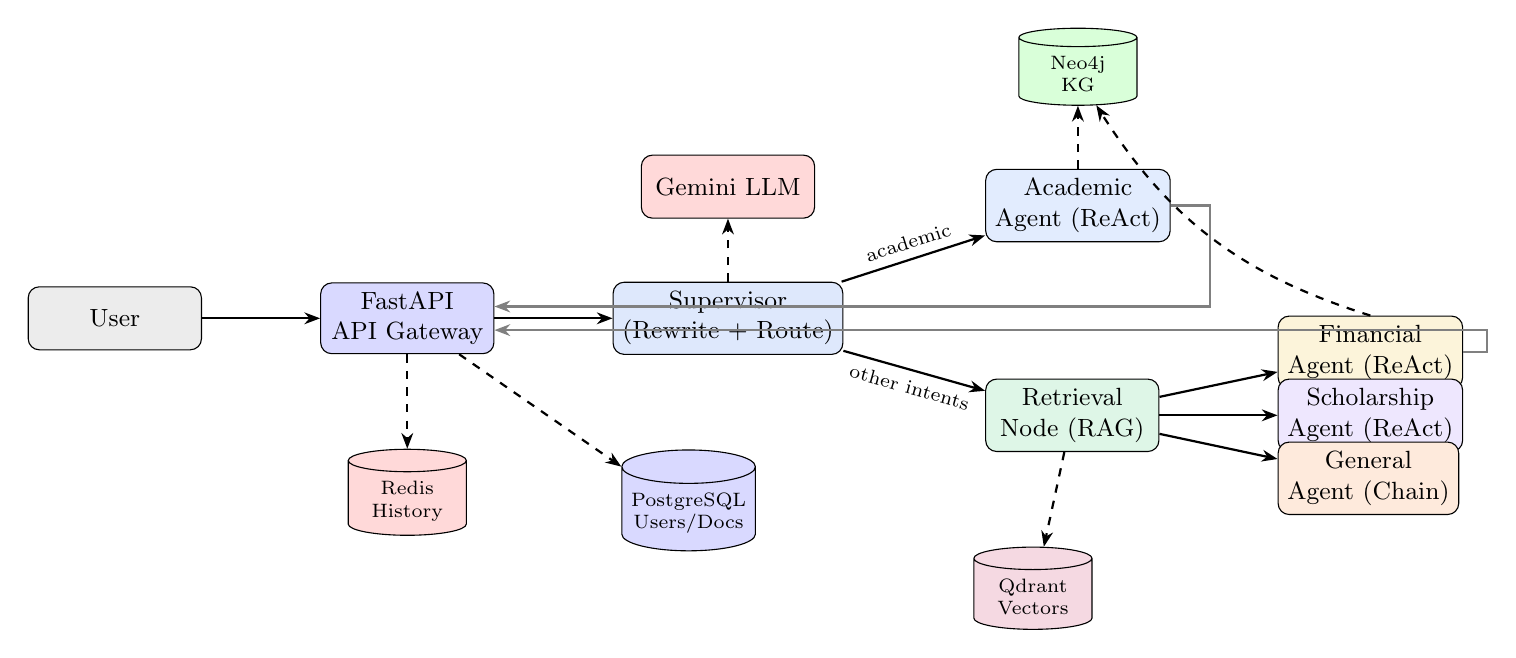
\begin{tikzpicture}[
    node distance=0.8cm and 1.2cm,
    every node/.style={font=\small},
    block/.style={rectangle, draw, rounded corners, minimum height=0.8cm, minimum width=2.2cm, align=center, fill=#1!15},
    block/.default=blue,
    db/.style={cylinder, draw, shape border rotate=90, aspect=0.25, minimum height=0.7cm, minimum width=1.5cm, fill=#1!15, align=center, font=\scriptsize},
    db/.default=gray,
    arrow/.style={-{Stealth[length=2mm]}, thick},
    dasharrow/.style={-{Stealth[length=2mm]}, thick, dashed},
]

% User
\node[block=gray] (user) {User};

% API Layer
\node[block=blue, right=1.5cm of user] (api) {FastAPI\\API Gateway};

% Supervisor
\node[block=supervisorblue, right=1.5cm of api] (sup) {Supervisor\\(Rewrite + Route)};

% Agents row
\node[block=academicblue, above right=0.5cm and 1.8cm of sup] (acad) {Academic\\Agent (ReAct)};
\node[block=retrievalgreen, below right=0.3cm and 1.8cm of sup] (ret) {Retrieval\\Node (RAG)};

% Post-retrieval agents
\node[block=financialyellow, right=1.5cm of ret, yshift=0.8cm] (fin) {Financial\\Agent (ReAct)};
\node[block=scholarshippurple, right=1.5cm of ret, yshift=-0.0cm] (sch) {Scholarship\\Agent (ReAct)};
\node[block=generalorange, right=1.5cm of ret, yshift=-0.8cm] (gen) {General\\Agent (Chain)};

% Databases
\node[db=red, below=1.2cm of api] (redis) {Redis\\History};
\node[db=blue, below=1.2cm of sup, xshift=-0.5cm] (pg) {PostgreSQL\\Users/Docs};
\node[db=purple, below=1.2cm of ret, xshift=-0.5cm] (qdrant) {Qdrant\\Vectors};
\node[db=green, above=0.8cm of acad] (neo4j) {Neo4j\\KG};

% LLM
\node[block=red, above=0.8cm of sup] (llm) {Gemini LLM};

% Arrows
\draw[arrow] (user) -- (api);
\draw[arrow] (api) -- (sup);
\draw[arrow] (sup) -- node[above, font=\scriptsize, sloped]{academic} (acad);
\draw[arrow] (sup) -- node[below, font=\scriptsize, sloped]{other intents} (ret);
\draw[arrow] (ret) -- (fin);
\draw[arrow] (ret) -- (sch);
\draw[arrow] (ret) -- (gen);

% DB connections
\draw[dasharrow] (api) -- (redis);
\draw[dasharrow] (api) -- (pg);
\draw[dasharrow] (ret) -- (qdrant);
\draw[dasharrow] (acad) -- (neo4j);
\draw[dasharrow] (fin.north) to[bend left=20] (neo4j);
\draw[dasharrow] (sup) -- (llm);

% Response arrows
\draw[arrow, gray] (acad.east) -- ++(0.5,0) |- ([yshift=0.15cm]api.east);
\draw[arrow, gray] (fin.east) -- ++(0.3,0) |- ([yshift=-0.15cm]api.east);

\end{tikzpicture}
\caption{CTU-Chat system architecture. The Supervisor routes queries to either the Academic Agent (direct Neo4j access) or the Retrieval Node (hybrid RAG), which then dispatches context to domain-specific agents. Dashed lines indicate data-store connections.}
\label{fig:architecture}
\end{figure}

The infrastructure layer comprises four Docker-containerized services:
\begin{itemize}
    \item \textbf{Qdrant} (v1.18.1): Vector database storing 768-dimensional child-chunk embeddings with cosine distance for dense retrieval.
    \item \textbf{Redis} (v7): In-memory cache for recent conversation history (bounded to 5 messages for context, 50 for session).
    \item \textbf{PostgreSQL} (v15): Relational storage for users, sessions, long-term chat history, parent documents, and metadata.
    \item \textbf{Neo4j} (v5.20): Graph database modeling academic programs, courses, prerequisites, and tuition structures.
\end{itemize}

The primary LLM is \texttt{gemini-3.5-flash-lite} for supervisor routing and all agent generation. A secondary \texttt{gemini-3.1-flash-lite} model handles query rewriting for lower latency and cost.

\subsection{Asymmetric Multi-Agent Design}
\label{sec:asymmetric}

A central contribution of CTU-Chat is its \emph{asymmetric} allocation of agent autonomy. Unlike homogeneous architectures where every agent runs a full ReAct loop, we match cognitive complexity to query requirements:

\begin{table}[t]
\centering
\caption{Asymmetric agent design: each agent receives autonomy proportional to its domain complexity.}
\label{tab:agents}
\small
\begin{tabular}{@{}lllll@{}}
\toprule
\textbf{Agent} & \textbf{Type} & \textbf{Tools} & \textbf{Data Source} & \textbf{Via Retrieval?} \\
\midrule
Academic   & ReAct (full)            & 6 Neo4j tools & Knowledge Graph & No \\
Financial  & ReAct (context-bounded) & 3 tools       & RAG + Neo4j     & Yes \\
Scholarship & ReAct (context-bounded) & 1 tool       & RAG context     & Yes \\
General    & Zero-shot chain         & None          & RAG context     & Yes \\
\bottomrule
\end{tabular}
\end{table}

\paragraph{Academic Agent.} This is the only fully autonomous agent. It operates a ReAct loop with six typed Neo4j tools: program lookup, program comparison, criteria-based search, prerequisite chain traversal, shared-course identification, and reverse course lookup. It bypasses document retrieval entirely, directly querying the knowledge graph through parameterized Cypher functions. This design exploits the natural isomorphism between graph traversal and the sequential reasoning pattern of LLMs.

\paragraph{Financial Agent.} This agent receives pre-retrieved RAG context from the Retrieval Node (filtered by IG-SRR lanes) and has access to three tools: graph-based tuition lookup, tuition regulation query, and a deterministic tuition calculator. The pre-loaded context constrains the agent's search space, preventing number hallucination on financial data while still allowing multi-step reasoning for complex calculations (e.g., ``calculate net tuition after 70\% exemption for Law program'').

\paragraph{Scholarship Agent.} Similar to the Financial Agent but with a single computational tool for GPA/conduct-based scholarship calculation. Its bounded autonomy reflects the simpler decision space of scholarship queries.

\paragraph{General Agent.} Implemented as a simple \texttt{prompt | LLM | StrOutputParser()} chain with \emph{zero} tools and \emph{no} reasoning loop. This agent handles open-ended policy questions where a single LLM call over retrieved context suffices. By eliminating the ReAct overhead (3--5 LLM calls per query), this agent achieves minimal latency for the most common query type.

This asymmetric design applies the Principle of Least Privilege to cognitive resources: agents receive only the autonomy they need, reducing token consumption and latency while maintaining answer quality where complex reasoning is required.

\subsection{Intent-Guided Subspace Retrieval Routing (IG-SRR)}
\label{sec:igssr}

The second core contribution is IG-SRR, a coupled mechanism that unifies intent classification with retrieval space partitioning. The Supervisor performs two decisions in a \emph{single} LLM call via structured output:

\begin{equation}
    f_{\text{route}}(q, h) \to (\text{next\_agent}, \text{intent})
    \label{eq:route}
\end{equation}

where $q$ is the (potentially rewritten) query, $h$ is the bounded conversation history, \texttt{next\_agent}~$\in$~\{academic, financial, scholarship, general\} selects the processing agent, and \texttt{intent}~$\in$~\{actual\_tuition, exemption\_basis, exemption\_policy, calculation, scholarship, student\_loan, academic\_program, \ldots\} selects the \emph{document subspace}.

Each intent maps to one or more \emph{Deterministic Retrieval Lanes}---metadata filter specifications that constrain both Qdrant dense search and BM25 sparse search:

\begin{equation}
    \mathcal{A}_l(q) = \{e \mid \text{status}(e) = \text{active},\; \text{domain}(e) = d_l,\; \text{kind}(e) = k_l,\; \text{fee}(e) = f_l\}
    \label{eq:lane}
\end{equation}

For example, the intent \texttt{calculation} activates three concurrent lanes: \texttt{actual\_tuition}, \texttt{exemption\_basis}, and \texttt{exemption\_policy}, ensuring the agent receives all document types needed for a complete financial computation. This one-to-many intent-to-lane mapping is a key novelty: the LLM predicts the \emph{nature} of required documents rather than extracting named entities for filtering.

Table~\ref{tab:lanes} shows the complete intent-to-lane mapping.

\begin{table}[t]
\centering
\caption{Intent-to-lane mapping in the IG-SRR mechanism.}
\label{tab:lanes}
\small
\begin{tabular}{@{}llp{5cm}@{}}
\toprule
\textbf{Intent} & \textbf{Lanes Activated} & \textbf{Documents Retrieved} \\
\midrule
actual\_tuition & actual\_tuition & Actual tuition rate tables \\
exemption\_basis & exemption\_basis & Exemption calculation bases \\
exemption\_policy & exemption\_policy & Exemption policy documents \\
calculation & actual + basis + policy & All three for computation \\
both / ambiguous & actual + basis & Both rate tables \\
scholarship & scholarship & Scholarship documents \\
student\_loan & student\_loan & Student loan documents \\
academic\_program & (empty) & Uses Neo4j tools directly \\
other & default (no filter) & Global search \\
\bottomrule
\end{tabular}
\end{table}

\subsection{Hybrid Retrieval Pipeline}
\label{sec:hybrid}

The retrieval pipeline operates \emph{within} the subspace defined by IG-SRR lanes:

\paragraph{Step 1: Document Ingestion and Parent-Child Chunking.}
Source documents (Markdown from manual curation or LlamaParse OCR) are split into parent sections (2,800-character limit, 100-character overlap) and child chunks (400 characters, 50-character overlap). A table-aware splitter repeats headers in every child chunk to preserve column semantics. Parent content is stored in PostgreSQL; child embeddings (768-dimensional, from \texttt{bkai-foundation-models/vietnamese-bi-encoder}) are indexed in Qdrant.

\paragraph{Step 2: Lane-Filtered Hybrid Search.}
For a given query $q$ and lane set $L$:
\begin{itemize}
    \item \textbf{Dense search}: Qdrant retrieves child chunks by cosine similarity, filtered by lane metadata.
    \item \textbf{Sparse search}: BM25 (with PyVi Vietnamese tokenization, $k_1\!=\!1.5$, $b\!=\!0.75$) retrieves children, filtered by the same lane metadata.
    \item \textbf{Parent aggregation}: Children are grouped by parent ID; the maximum child score represents each parent.
\end{itemize}

\paragraph{Step 3: RRF Fusion.}
Parent lists from dense and sparse branches are fused using Equation~\ref{eq:rrf} with $k=60$.

\paragraph{Step 4: Cross-Encoder Reranking with Temporal Tie-Break.}
The \texttt{BAAI/bge-reranker-v2-m3} cross-encoder rescores the top 15 fused parents. Within a score tolerance of 0.05, documents are reordered by timestamp (newer first), implementing a bounded temporal tie-break that preserves source coverage without degrading relevance ranking.

\subsection{Knowledge Graph Integration}
\label{sec:kg}

The Neo4j knowledge graph models the CTU academic domain with nodes for Programs, Courses, and structural relationships (prerequisites, electives, shared courses). Rather than exposing the graph schema to the LLM for raw Cypher generation, we implement six \textbf{typed Python tool functions}:

\begin{enumerate}
    \item \texttt{tra\_cuu\_nganh}: Look up detailed program information
    \item \texttt{so\_sanh\_nganh}: Compare two programs side-by-side
    \item \texttt{tim\_nganh}: Search programs by criteria
    \item \texttt{xem\_chuoi\_tien\_quyet}: Traverse prerequisite chains
    \item \texttt{mon\_chung\_giua\_nganh}: Find shared courses between programs
    \item \texttt{tim\_nganh\_co\_mon}: Reverse lookup: which programs teach course X
\end{enumerate}

Each tool encapsulates a validated Cypher query with parameterized inputs, eliminating the risk of schema hallucination. The Financial Agent additionally accesses two graph tools (\texttt{tra\_cuu\_hoc\_phi\_graph} for tuition lookup and \texttt{tra\_cuu\_quy\_dinh\_hoc\_phi} for fee regulations) and one deterministic calculator (\texttt{tinh\_toan\_hoc\_phi}).

\subsection{Query Processing Algorithm}
\label{sec:algorithm}

Algorithm~\ref{alg:supervisor} describes the Supervisor routing logic, which performs query rewriting and intent-based routing in a unified pipeline.

\begin{algorithm}[t]
\caption{Supervisor Node: Query Rewrite and Routing}
\label{alg:supervisor}
\begin{algorithmic}[1]
\Require Query $q$, chat history $h$, rewrite LLM $M_r$, routing LLM $M_s$
\Ensure Updated state with \texttt{search\_query}, \texttt{next\_agent}, \texttt{intent}
\Statex
\Function{SupervisorNode}{$q, h$}
    \State $q_s \gets q$ \Comment{Default: use original query}
    \If{\Call{ShouldRewrite}{$q, h$}} \Comment{Contains pronouns, ellipsis}
        \State $q_r \gets M_r(q, h[-1])$ \Comment{Rewrite with previous turn}
        \If{\Call{ValidateRewrite}{$q_r, q$}} \Comment{No new entities/numbers}
            \State $q_s \gets q_r$
        \EndIf
    \EndIf
    \State $(\text{agent}, \text{intent}) \gets M_s.\text{structured\_output}(q_s, h)$
    \State \Return $\{$search\_query: $q_s$, next\_agent: agent, intent: intent$\}$
\EndFunction
\end{algorithmic}
\end{algorithm}

Algorithm~\ref{alg:igssr} formalizes the IG-SRR lane selection and retrieval process.

\begin{algorithm}[t]
\caption{Intent-Guided Subspace Retrieval Routing (IG-SRR)}
\label{alg:igssr}
\begin{algorithmic}[1]
\Require Search query $q_s$, routing decision $(agent, intent)$
\Ensure Retrieved context $C$, retrieval instruction $I$
\Statex
\Function{RetrievalNode}{$q_s, agent, intent$}
    \If{$agent = $ ``academic''}
        \State \Return $\emptyset$ \Comment{Academic agent uses Neo4j directly}
    \EndIf
    \State $L \gets \Call{BuildLanes}{intent}$ \Comment{Intent $\to$ lane set}
    \State $C_{\text{struct}} \gets \emptyset$
    \If{$agent = $ ``financial''}
        \State $C_{\text{struct}} \gets \Call{Neo4jLookup}{q_s}$ \Comment{Graph structured data}
        \If{$C_{\text{struct}} = \emptyset$}
            \State $C_{\text{struct}} \gets \Call{JSONCatalogFallback}{q_s}$
        \EndIf
    \EndIf
    \ForAll{lane $l \in L$}
        \State $D_l \gets \Call{DenseSearch}{q_s, \text{filter}(l)}$ \Comment{Qdrant}
        \State $S_l \gets \Call{SparseSearch}{q_s, \text{filter}(l)}$ \Comment{BM25}
        \State $P_l \gets \Call{ParentAggregate}{D_l \cup S_l}$
    \EndFor
    \State $F \gets \Call{RRFFusion}{\bigcup_l P_l}$ \Comment{Eq.~\ref{eq:rrf}}
    \State $R \gets \Call{Rerank}{F, q_s}$ \Comment{Cross-encoder + tie-break}
    \State $C \gets C_{\text{struct}} \cup \Call{BuildContext}{R}$
    \State $I \gets \Call{BuildInstruction}{intent, L}$
    \State \Return $(C, I)$
\EndFunction
\end{algorithmic}
\end{algorithm}

\subsection{System Activity Flow}
\label{sec:flowchart}

Figure~\ref{fig:flowchart} presents the complete activity flowchart of CTU-Chat, showing the decision points where the system branches based on query type, intent classification, and data source selection.

\begin{figure}[t]
\centering
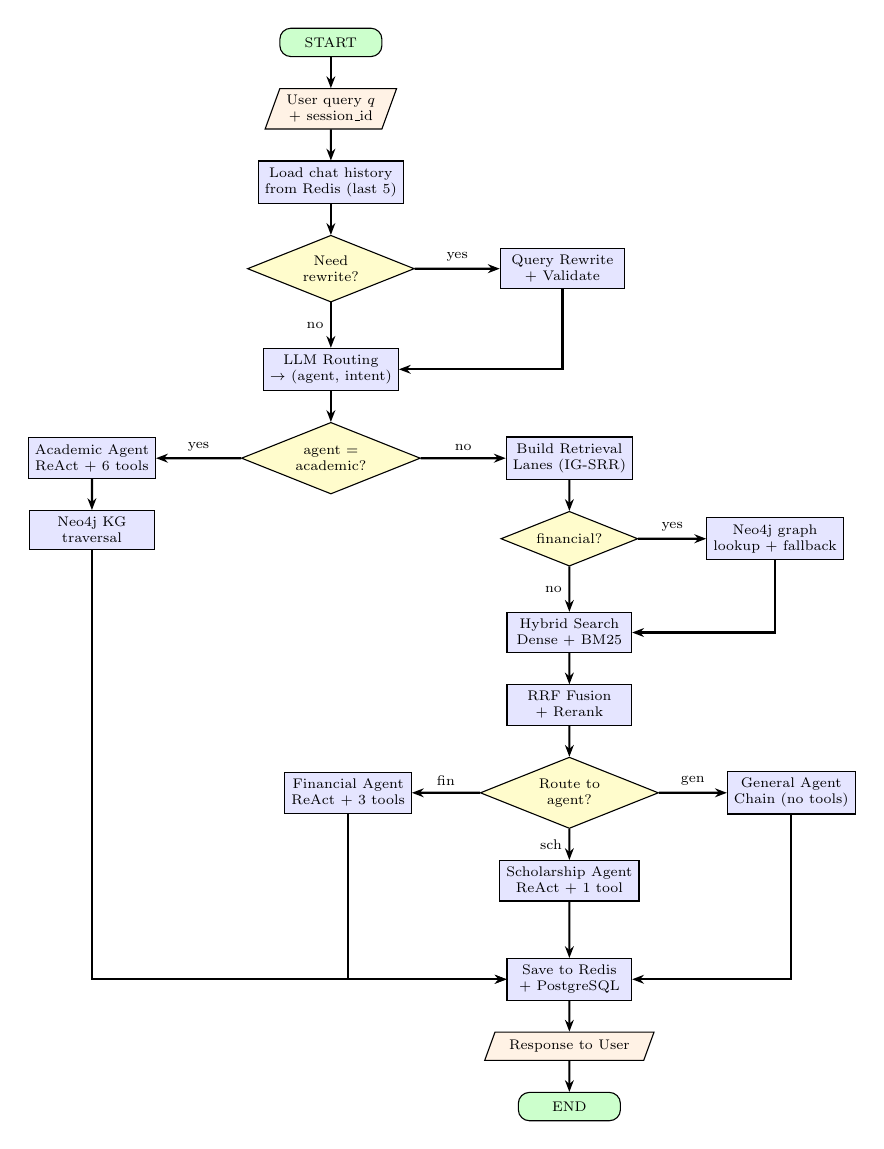
\begin{tikzpicture}[
    scale=0.72, transform shape,
    node distance=0.55cm,
    every node/.style={font=\scriptsize},
    startstop/.style={rectangle, rounded corners, draw, fill=green!20, minimum width=1.8cm, minimum height=0.5cm, align=center},
    process/.style={rectangle, draw, fill=blue!10, minimum width=2.2cm, minimum height=0.5cm, align=center},
    decision/.style={diamond, draw, fill=yellow!20, minimum width=1.2cm, minimum height=0.5cm, align=center, aspect=2.5},
    io/.style={trapezium, trapezium left angle=70, trapezium right angle=110, draw, fill=orange!10, minimum width=1.8cm, minimum height=0.5cm, align=center},
    arrow/.style={-{Stealth[length=1.5mm]}, thick},
]

% Start
\node[startstop] (start) {START};
\node[io, below=of start] (input) {User query $q$\\+ session\_id};
\node[process, below=of input] (history) {Load chat history\\from Redis (last 5)};
\node[decision, below=of history] (rewrite) {Need\\rewrite?};
\node[process, right=1.5cm of rewrite] (dorewrite) {Query Rewrite\\+ Validate};
\node[process, below=0.8cm of rewrite] (route) {LLM Routing\\$\to$ (agent, intent)};
\node[decision, below=of route] (isacad) {agent =\\academic?};

% Academic branch
\node[process, left=1.5cm of isacad] (acadagent) {Academic Agent\\ReAct + 6 tools};
\node[process, below=of acadagent] (neo4j) {Neo4j KG\\traversal};

% Retrieval branch
\node[process, right=1.5cm of isacad] (lanes) {Build Retrieval\\Lanes (IG-SRR)};
\node[decision, below=of lanes] (isfin) {financial?};
\node[process, right=1.2cm of isfin] (graphlookup) {Neo4j graph\\lookup + fallback};
\node[process, below=0.8cm of isfin] (hybrid) {Hybrid Search\\Dense + BM25};
\node[process, below=of hybrid] (rrf) {RRF Fusion\\+ Rerank};
\node[decision, below=of rrf] (whichagent) {Route to\\agent?};

% Final agents
\node[process, left=1.2cm of whichagent] (finagent) {Financial Agent\\ReAct + 3 tools};
\node[process, below=of whichagent] (schagent) {Scholarship Agent\\ReAct + 1 tool};
\node[process, right=1.2cm of whichagent] (genagent) {General Agent\\Chain (no tools)};

% Output
\node[process, below=1cm of schagent] (save) {Save to Redis\\+ PostgreSQL};
\node[io, below=of save] (output) {Response to User};
\node[startstop, below=of output] (end) {END};

% Arrows
\draw[arrow] (start) -- (input);
\draw[arrow] (input) -- (history);
\draw[arrow] (history) -- (rewrite);
\draw[arrow] (rewrite) -- node[above]{yes} (dorewrite);
\draw[arrow] (rewrite) -- node[left]{no} (route);
\draw[arrow] (dorewrite) |- (route);
\draw[arrow] (route) -- (isacad);
\draw[arrow] (isacad) -- node[above]{yes} (acadagent);
\draw[arrow] (isacad) -- node[above]{no} (lanes);
\draw[arrow] (acadagent) -- (neo4j);
\draw[arrow] (lanes) -- (isfin);
\draw[arrow] (isfin) -- node[above]{yes} (graphlookup);
\draw[arrow] (isfin) -- node[left]{no} (hybrid);
\draw[arrow] (graphlookup) |- (hybrid);
\draw[arrow] (hybrid) -- (rrf);
\draw[arrow] (rrf) -- (whichagent);
\draw[arrow] (whichagent) -- node[above]{fin} (finagent);
\draw[arrow] (whichagent) -- node[left]{sch} (schagent);
\draw[arrow] (whichagent) -- node[above]{gen} (genagent);

% All agents to save
\draw[arrow] (neo4j) |- (save);
\draw[arrow] (finagent) |- (save);
\draw[arrow] (schagent) -- (save);
\draw[arrow] (genagent) |- (save);

\draw[arrow] (save) -- (output);
\draw[arrow] (output) -- (end);

\end{tikzpicture}
\caption{Complete activity flowchart of CTU-Chat. Decision diamonds show branching logic: query rewrite validation, academic vs.\ retrieval routing, financial graph pre-lookup, and final agent dispatch.}
\label{fig:flowchart}
\end{figure}

The flowchart illustrates several key design decisions:
\begin{itemize}
    \item \textbf{Academic queries bypass retrieval entirely}, going directly to the Neo4j-powered ReAct agent---this eliminates unnecessary vector search latency for relational queries.
    \item \textbf{Financial queries receive both graph-structured context and RAG documents}, ensuring the agent has exact figures from Neo4j alongside explanatory policy text from the document corpus.
    \item \textbf{General queries follow the shortest path}: retrieval $\to$ zero-shot chain, requiring only two LLM calls total (one for routing, one for generation).
\end{itemize}

\paragraph{Data Characteristics and Retrieval Strategy Justification.}
The choice of retrieval modality is driven by the inherent structure of CTU data:

\begin{itemize}
    \item \textbf{Academic programs} (curricula, prerequisites, shared courses): inherently \emph{relational} data with graph topology $\to$ Neo4j Knowledge Graph with graph traversal tools.
    \item \textbf{Tuition and fees}: \emph{tabular} data requiring numerical precision $\to$ Hybrid RAG with lane-filtered structured context + deterministic calculation tools.
    \item \textbf{Policies and regulations}: \emph{narrative} text requiring semantic understanding $\to$ Dense vector search for semantic similarity + BM25 for keyword matching on Vietnamese compound nouns.
    \item \textbf{Scholarships and loans}: mix of \emph{policy text} and \emph{computational rules} $\to$ RAG context + specialized calculation tools.
\end{itemize}

This analysis justifies when to use keyword search (BM25: exact terms, regulation codes), when to use semantic search (Dense: paraphrased questions, synonyms), and when to use graph queries (Neo4j: multi-hop relational lookups).


% ============================================================
% 4. EXPERIMENTAL RESULTS
% ============================================================
\section{Experimental Results}
\label{sec:experiments}

\subsection{Experimental Dataset}
\label{sec:dataset}

We constructed a Vietnamese-language evaluation dataset of 100 questions balanced across four domains: exemption and social support (25), tuition (25), student loans (25), and scholarships (25). Each question includes:
\begin{itemize}
    \item The \textbf{question text} in Vietnamese, reflecting real student queries collected from CTU counseling channels and FAQ pages.
    \item An \textbf{expected answer} with key factual elements that a correct response must contain.
    \item The \textbf{expected source filename(s)} identifying which document(s) should be retrieved.
    \item The \textbf{domain label} for stratified analysis.
\end{itemize}

The corpus comprises 50 Markdown policy and tuition documents under \texttt{data/markdown} and 114 academic-program Markdown files under \texttt{data/markdown\_graph}. The active Qdrant collection contains 1,303 vector points. Documents were curated from official CTU publications, with metadata including domain, content kind, fee kind, academic year, and active/inactive status.

% TODO: Add more detail about dataset construction process (contribution to research)

\subsection{Experimental Tools}
\label{sec:tools}

Table~\ref{tab:tools} summarizes the software stack used in experiments.

\begin{table}[t]
\centering
\caption{Experimental tools and versions.}
\label{tab:tools}
\small
\begin{tabular}{@{}ll@{}}
\toprule
\textbf{Component} & \textbf{Implementation} \\
\midrule
Web Framework & FastAPI \\
Agent Orchestration & LangGraph (StateGraph) \\
Dense Vector Store & Qdrant v1.18.1 (768-dim, cosine) \\
Sparse Retrieval & BM25s + PyVi tokenizer \\
Graph Database & Neo4j v5.20.0 \\
Cross-Encoder Reranker & BAAI/bge-reranker-v2-m3 \\
Session Store & Redis v7 \\
Persistent Store & PostgreSQL v15 \\
Primary LLM & Gemini gemini-3.5-flash-lite \\
Rewrite LLM & Gemini gemini-3.1-flash-lite \\
Embedding Model & bkai-foundation-models/vietnamese-bi-encoder \\
Evaluation Framework & RAGAS + custom LLM judge \\
\bottomrule
\end{tabular}
\end{table}

\subsection{Evaluation Metrics}
\label{sec:metrics}

We employ three categories of metrics:

\paragraph{Retrieval Metrics.} Precision at 5 (P@5), Recall at 5 (Recall@5), and Mean Reciprocal Rank (MRR):
\begin{equation}
    \text{P@5} = \frac{|\text{Rel} \cap \text{Top5}|}{5}, \quad
    \text{Recall@5} = \frac{|\text{Rel} \cap \text{Top5}|}{|\text{Rel}|}, \quad
    \text{MRR} = \frac{1}{N}\sum_{q=1}^{N}\frac{1}{\text{rank}^{\text{first}}_q}
    \label{eq:metrics}
\end{equation}

\paragraph{Answer Quality Metrics (RAGAS).} Answer Relevance, Context Recall, Context Precision, and Answer Correctness, evaluated using an LLM-as-a-judge approach with the judge model and prompt configuration reported alongside results.

\paragraph{System Metrics.} Chat LLM-judge pass rate (threshold 0.55), tool-call path selection accuracy, argument validity, result correctness, end-to-end tool success rate, and reranker expected-source coverage.

\subsection{Experimental Scenarios}
\label{sec:scenarios}

We design three experimental scenarios, each corresponding to a distinct evaluation table.

\subsubsection{Scenario 1: Retrieval Ablation}
This scenario isolates the contribution of each retrieval component by comparing four configurations on the same 100-question dataset. Table~\ref{tab:retrieval} presents the planned metrics.

\begin{table}[t]
\centering
\caption{Scenario 1: Retrieval ablation---isolating dense, sparse, hybrid, and reranked retrieval. All values are pending controlled experiments.}
\label{tab:retrieval}
\small
\begin{tabular}{@{}lccccccc@{}}
\toprule
\textbf{Configuration} & \textbf{P@5} & \textbf{R@5} & \textbf{MRR} & \textbf{Ans.Rel} & \textbf{Ctx.Rec} & \textbf{Ctx.Prec} & \textbf{Ans.Corr} \\
\midrule
Dense only          & -- & -- & -- & -- & -- & -- & -- \\
Sparse only (BM25)  & -- & -- & -- & -- & -- & -- & -- \\
Hybrid RRF          & -- & -- & -- & -- & -- & -- & -- \\
Hybrid RRF + Rerank & -- & -- & -- & -- & -- & -- & -- \\
\bottomrule
\end{tabular}
\end{table}

This ablation will answer \textbf{RQ3} by quantifying whether hybrid retrieval with reranking outperforms single-mode approaches. The existing codebase provides \texttt{evaluate\_ragas.py} and \texttt{score\_ragas.py} for automated execution.

\subsubsection{Scenario 2: Graph and Agent Ablation}
This scenario evaluates the knowledge graph integration and routing mechanism independently from document retrieval. Table~\ref{tab:agent} presents the planned metrics.

\begin{table}[t]
\centering
\caption{Scenario 2: Graph and agent ablation---evaluating routing accuracy, tool validity, and graph query quality. All values are pending.}
\label{tab:agent}
\small
\begin{tabular}{@{}lcccc@{}}
\toprule
\textbf{Variant} & \textbf{Route Acc.} & \textbf{Tool Valid.} & \textbf{Graph Metric} & \textbf{Answer Metrics} \\
\midrule
Graph only          & n/a     & --      & --      & -- \\
Fixed route + Hybrid & --     & --      & n/a     & -- \\
Supervisor + Hybrid  & --     & --      & n/a     & -- \\
Full system          & --     & --      & --      & -- \\
\bottomrule
\end{tabular}
\end{table}

This ablation will address \textbf{RQ1} by comparing supervisor-based routing against fixed routing, and \textbf{RQ2} by evaluating whether IG-SRR lane filtering improves answer quality.

\subsubsection{Scenario 3: Full System Evaluation}
This scenario reports the end-to-end system performance using the complete CTU-Chat pipeline. Table~\ref{tab:fullsystem} presents results from the current implementation.

\begin{table}[t]
\centering
\caption{Scenario 3: Full system evaluation---recorded implementation metrics.}
\label{tab:fullsystem}
\small
\begin{tabular}{@{}llrl@{}}
\toprule
\textbf{Evaluation} & \textbf{Num./Denom.} & \textbf{Result} & \textbf{Interpretation} \\
\midrule
Chat judge pass rate     & 91/100 & 91.00\%  & Latest 100-question run \\
Chat mean judge score    & --     & 81.35\%  & LLM judge score \\
Chat API errors          & 0/100  & 0        & HTTP/API layer \\
Tool path selection      & 30/30  & 100.00\% & Three tool families \\
Tool argument validity   & 29/30  & 96.67\%  & One argument mismatch \\
Tool result correctness  & 30/30  & 100.00\% & Deterministic checks \\
Tool end-to-end cases    & 29/30  & 96.67\%  & Isolated sessions \\
Reranker source hit      & 80/80  & 100.00\% & All three reranker variants \\
\midrule
\multicolumn{4}{@{}l@{}}{\textit{Domain breakdown (pass rate):}} \\
\quad Exemption/Social support & 25/25 & 100\% & \\
\quad Tuition                  & 23/25 & 92\%  & \\
\quad Scholarship              & 23/25 & 92\%  & \\
\quad Student loans             & 20/25 & 80\%  & \\
\bottomrule
\end{tabular}
\end{table}

The full system achieved 91\% overall pass rate with 100\% expected-source coverage across all reranker variants. Tool-calling accuracy reached 96.67\%, with the single failure attributed to argument selection in the scholarship calculation tool. Domain analysis reveals strongest performance on exemption/social-support questions (100\%) and weakest on student-loan queries (80\%), consistent with the corpus containing overlapping loan regulations that challenge semantic disambiguation.

\subsection{Discussion}
\label{sec:discussion}

The implementation results demonstrate that the asymmetric multi-agent architecture with IG-SRR produces a functional system with high overall quality, but several observations warrant discussion.

\paragraph{Strengths.}
The separation of concerns---exact catalog lookups and arithmetic in structured tools, semantic retrieval for policy context, and graph queries for relational data---prevents the failure modes common in monolithic RAG systems. The 100\% tool-call selection accuracy confirms that the typed tool abstraction successfully eliminates schema hallucination on Neo4j queries. The reranker A/B experiment shows that all three scoring variants maintain complete source coverage, validating the IG-SRR lane filtering approach.

\paragraph{Domain-specific Performance Variation.}
Student-loan queries underperformed other domains (80\% vs.\ 92--100\%). This pattern is consistent with a corpus containing multiple overlapping loan regulations from different years, where the current lane filter (domain-level only) cannot distinguish between active and superseded provisions as effectively as the more granular tuition lane filters.

\paragraph{Limitations.}
\begin{itemize}
    \item The 100-question benchmark uses an LLM judge rather than paired human evaluation, limiting the strength of accuracy claims.
    \item Source-hit ranking is not equivalent to answer faithfulness; a system can retrieve the correct source but still generate an incorrect answer.
    \item The corpus contains multiple document versions and inactive records; metadata quality directly affects retrieval precision.
    \item Gap~4 (temporal degradation) remains unaddressed beyond basic \texttt{academic\_year} filtering; bi-temporal graph support is needed for production deployment.
    \item The rewrite guard is heuristic, and session memory is bounded by list length rather than a learned memory policy.
    \item No statistically powered ablation with confidence intervals has been conducted; the planned experiments in Tables~\ref{tab:retrieval} and~\ref{tab:agent} will address this.
\end{itemize}

% ============================================================
% 5. CONCLUSION
% ============================================================
\section{Conclusion}
\label{sec:conclusion}

This paper presented CTU-Chat, a Vietnamese university counseling system that addresses three of the five critical research gaps in Agentic GraphRAG systems for education. The \emph{Asymmetric Multi-Agent} architecture matches agent autonomy to domain complexity, reducing computational overhead on simple queries while preserving multi-step reasoning for complex ones. \emph{Intent-Guided Subspace Retrieval Routing} (IG-SRR) couples intent classification with deterministic metadata lane filters, confining hybrid retrieval to ontologically correct document subspaces and improving retrieval precision. \emph{Typed Knowledge Graph tools} eliminate schema hallucination by replacing raw Cypher generation with safe, parameterized Python functions.

Preliminary evaluation on a 100-question Vietnamese benchmark demonstrates 91\% LLM-judge pass rate, 96.67\% tool-calling accuracy, and 100\% expected-source coverage. Domain analysis reveals strong performance across most query types, with student-loan queries identified as the primary area for improvement due to overlapping regulations in the corpus.

The central engineering insight is the value of \emph{separation of concerns}: exact lookups and arithmetic belong to structured components, semantic and lexical retrieval complement each other within lane-bounded subspaces, and graph queries should be used where the question is inherently relational. This asymmetric design philosophy offers a principled alternative to the homogeneous multi-agent architectures prevalent in current literature.

\paragraph{Future Work.}
Immediate priorities include completing the controlled retrieval ablations (Table~\ref{tab:retrieval}) and agent ablation experiments (Table~\ref{tab:agent}), conducting paired human evaluation alongside LLM-judge scoring, implementing bi-temporal graph support for temporal knowledge management (Gap~4), and developing a comprehensive multi-agent evaluation framework with execution-grounded metrics (Gap~5). We also plan to extend the benchmark to cover academic-program queries and to deploy CTU-Chat in a production pilot with real student users.

% ============================================================
% REFERENCES
% ============================================================
\begin{thebibliography}{10}

\bibitem{lewis2020rag}
Lewis, P., Perez, E., Piktus, A., et al.:
Retrieval-augmented generation for knowledge-intensive NLP tasks.
Advances in Neural Information Processing Systems \textbf{33}, 9459--9474 (2020)

\bibitem{robertson2009bm25}
Robertson, S., Zaragoza, H.:
The probabilistic relevance framework: BM25 and beyond.
Foundations and Trends in Information Retrieval \textbf{3}(4), 333--389 (2009)

\bibitem{cormack2009rrf}
Cormack, G.V., Clarke, C.L.A., Buettcher, S.:
Reciprocal rank fusion outperforms condorcet and individual rank learning methods.
In: Proc.\ 32nd International ACM SIGIR Conference, pp.~758--759 (2009)

\bibitem{edge2024graphrag}
Edge, D., Trinh, H., Cheng, N., et al.:
From local to global: A graph RAG approach to query-focused summarization.
arXiv preprint arXiv:2404.16130 (2024)

\bibitem{yao2023react}
Yao, S., Zhao, J., Yu, D., et al.:
ReAct: Synergizing reasoning and acting in language models.
In: International Conference on Learning Representations (2023)

\bibitem{ma2025rebot}
Ma, T., La, T.T., Le Huu, L.T., et al.:
REBot: From RAG to CatRAG with semantic enrichment and graph routing.
arXiv preprint arXiv:2510.01800 (2025)

\bibitem{nogueira2020reranker}
Nogueira, R., Jiang, Z., Lin, J.:
Document ranking with a pretrained sequence-to-sequence model.
In: Findings of EMNLP (2020)

\bibitem{karag2024}
KA-RAG: Integrating Knowledge Graphs and Agentic Retrieval.
Applied Sciences \textbf{15}(23), 12547 (2024)

\bibitem{cyveract2024}
CyVerACT: An Agentic Cypher Translation Workflow over Knowledge Graphs.
ResearchGate (2024)

\bibitem{multiagent_university2025}
An Empirical Study of Multi-Agent RAG for Real-World University Applications.
arXiv:2507.11272 (2025)

\bibitem{langgraph_benchmark2024}
Benchmarking Multi-Agent Architectures.
LangChain Blog (2024)

\end{thebibliography}

\end{document}
